\documentclass[11pt,a4j]{jarticle}

\newcommand{\setcounters}[1] {
  \setcounter{equation}{#1}
  \setcounter{figure}{#1}
  \setcounter{table}{#1}
}

\newcommand{\unit}[1] {
  \hspace{1mm}\mathrm{[#1]}
}

\newcommand{\degc} {
  \hspace{1mm}\mathrm{[}{}^\circ\mathrm{C]}
}

\newcommand{\refig}[1]{図\ref{fig::#1}}
\newcommand{\refeq}[1]{式(\ref{eq::#1})}
\newcommand{\reftab}[1]{表\ref{tab::#1}}

\newcommand{\fig}[5] {
  \begin{figure}[#1]
    \begin{center}
      \includegraphics[width=#2\hsize]{#3}
    \end{center}
    \caption{#4}
    \label{fig::#5}
  \end{figure}
}

\makeatletter
\def\eq{\@ifstar\@eq\@@eq}
\def\@eq#1{\begin{equation*}#1\end{equation*}}
\def\@@eq#1#2{\begin{equation}#2\label{eq::#1}\end{equation}}
\makeatother

\newcommand{\diff}[2] {
  \frac{\mathrm{d}#1}{\mathrm{d}#2}
}

\newcommand{\pdiff}[2] {
  \frac{\partial #1}{\partial #2}
}


\newcommand{\ddt}[2][1] {
  \ifnum #1 < 2
    \frac{\mathrm{d}#2}{\mathrm{d}t}
  \else
    \frac{\mathrm{d}^#1#2}{\mathrm{d}t^#1}
  \fi
}

\newcommand{\e}[1] {
  \mathrm{e}^{#1}
}

\newcommand{\lparen}{(}
\catcode `( = \active
\newcommand{(}{\ifmmode\left\lparen\else\lparen\fi}

\newcommand{\rparen}{)}
\catcode `) = \active
\newcommand{)}{\ifmmode\right\rparen\else\rparen\fi}

\newcommand{\bmat}[1] {
  \begin{bmatrix} #1 \end{bmatrix}
}

% -- Package ---------------------------------------------------
\usepackage[dvipdfmx]{graphicx}
\usepackage{amsmath, amssymb}
\usepackage{bm}
\usepackage{fancyhdr}
\usepackage{here}
\usepackage{listings}
\usepackage{multirow}


% -- Margin Config ---------------------------------------------
\setlength{\textheight}{\paperheight}
\setlength{\topmargin}{4.6truemm} % 30mm(=1.0in+4.6mm)
\addtolength{\topmargin}{-\headheight}
\addtolength{\topmargin}{-\headsep}
\addtolength{\textheight}{-60truemm}

\setlength{\textwidth}{\paperwidth}
\setlength{\oddsidemargin}{-0.4truemm} % 25mm(=1.0in-0.4mm)
\setlength{\evensidemargin}{-0.4truemm}
\addtolength{\textwidth}{-50truemm}


% -- Renewcommand ----------------------------------------------
\renewcommand{\theequation}{\arabic{section}.\arabic{equation}}
\renewcommand{\thefigure}{\arabic{figure}}
\renewcommand{\thetable}{\thesection.\arabic{table}}
\renewcommand{\lstlistingname}{ソースコード}
\renewcommand{\headrulewidth}{0mm} % fancy
\renewcommand{\labelenumi}{(\arabic{enumi})}


% -- Config for fancy package ----------------------------------
\pagestyle{fancy}
\rhead{\thepage}
\lhead{}
\cfoot{}


% -- Config for package listings -------------------------------
\lstset{
  basicstyle={\ttfamily \small},
  breaklines=true,
  frame=trBL,
  numbers=left,
  numberstyle={\ttfamily \small},
}




\begin{document}
\begin{titlepage}

  \vspace*{25mm}

  \begin{center}
    {\huge 知能制御PBL\\}
    \vspace{10mm}
    {\Huge 第2回RCR中間報告\\}
    \vspace{20mm}
    {\Large 2018年6月6日}

    \vspace{15mm}

    {\LARGE 西田研究室\\}

    \vspace{15mm}

    {\Large
   13104042 烏谷崇大    \\
   14104055 佐々木秀将\\
   15104021 長田駿二郎\\
   15104026 川崎雄太朗\\
   15104050 坂元勇太    \\
   15104081 徳野将士    \\
   15104113 前田修一    \\
   15104117 右田明花    \\
   15104134 山福佳        \\
   17104311 横田篤紀    \\
}

  \end{center}

\end{titlepage}


\newpage
	\tableofcontents

\newpage
\section{目的}
	学部3年までに学習した制御理論や電気回路・情報工学の知識を使って,競技場内を自律的に走行するロボットの製作を行う.
	研究室で一丸となってプロジェクトを進行し,共同で課題を達成することの難しさや楽しさを学び,エンジニアとして仕事を進めるための素養を身に付ける.

\section{RCR (Robot Car Race) 2018}

\subsection{競技概要}
	ウレタンパネルを用いてレイアウトされる周回コースにおいて,格子模様のコントロールライン手前から走行開始してコントロールラインを3回通過後に停止するまでの時間を競うロボットカー(ロボカー)を製作する.

\subsection{コース}
	一辺$50\unit{cm}$の正方形及び扇形の黒色ウレタンパネルと白黒格子模様のコントロールライン付ウレタンパネルを組み合わせ,コースを構成する.
	なお,競技会当日までコースは公表されない.また,コースフェンスの高さが低いため,コースフェンスのコース側に高さ$10\unit{cm}$の壁を設置する.

\subsection{競技ルール}
	\begin{enumerate}
      \item コントロールライン手前からの走行開始からコントロールラインを3回通過後に停止するまでの時間を競う.
      \item 各チームあたり10分以内に最大3回走行し,最短時間の走行を評価する.
      \item コース2周以上走行すること.
      \item 競技会当日のコース試走は認めない.
      \item ロボカーがコース周囲の壁に接触した場合は失格とする.
      \item コース及び壁に物を設置したり,手を加えてはいけない.
      \item コース内に足を踏み入れないこと.
    \end{enumerate}

\newpage

\section{ROS (Robot Operating System)}
\subsection{ROSとは}
ROS(Robot Operating System)とはOpen Source Robotics Foundationによって管理されているソフトウェア開発者のロボット・アプリケーション作成を支援するフレームワークである.
具体的には,ハードウェア抽象化,デバイスドライバ,ライブラリ,視覚化ツール,メッセージ通信,パッケージ管理などが提供されている.つまりROSは汎用コンピュータ向けのOSではなく,汎用コンピュータ向けOS上で動作するメタOSとして捉えることができる\cite{kurazume}.

\refig{ros_topic}に示すようにROSではプロセス(実行プログラム)はノードという単位で扱い,ノード間の通信はトピックと呼ばれる``Publisher/Subscriber''モデルで実現される\cite{ogura}.

これにより,プログラミング言語や通信相手さえ意識することなく簡単にプロセス間通信を実現できる.
これは各ノード間のインタフェース,すなわちトピックの名前と型さえ決定すればノードごとに独立して開発を行うことができるという利点でもある.\\

以上の利点を考慮し,本研究室ではROSがインストール可能なマイコンボードであるRaspberryPi3 Model B上にROSをインストールして開発を進めていくこととした.

\begin{figure}[htb]
  \centering
    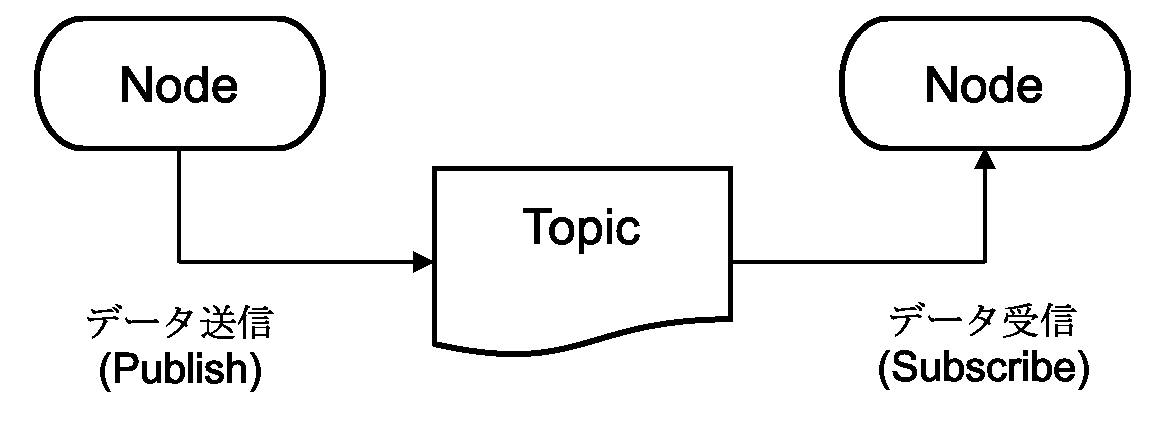
\includegraphics[width=0.5\hsize]{picture/eps/ros_topic.eps}
    \caption{ROSノードとトピックの概念}
    \label{fig::ros_topic}
\end{figure}



\begin{figure}[htb]
  \centering
    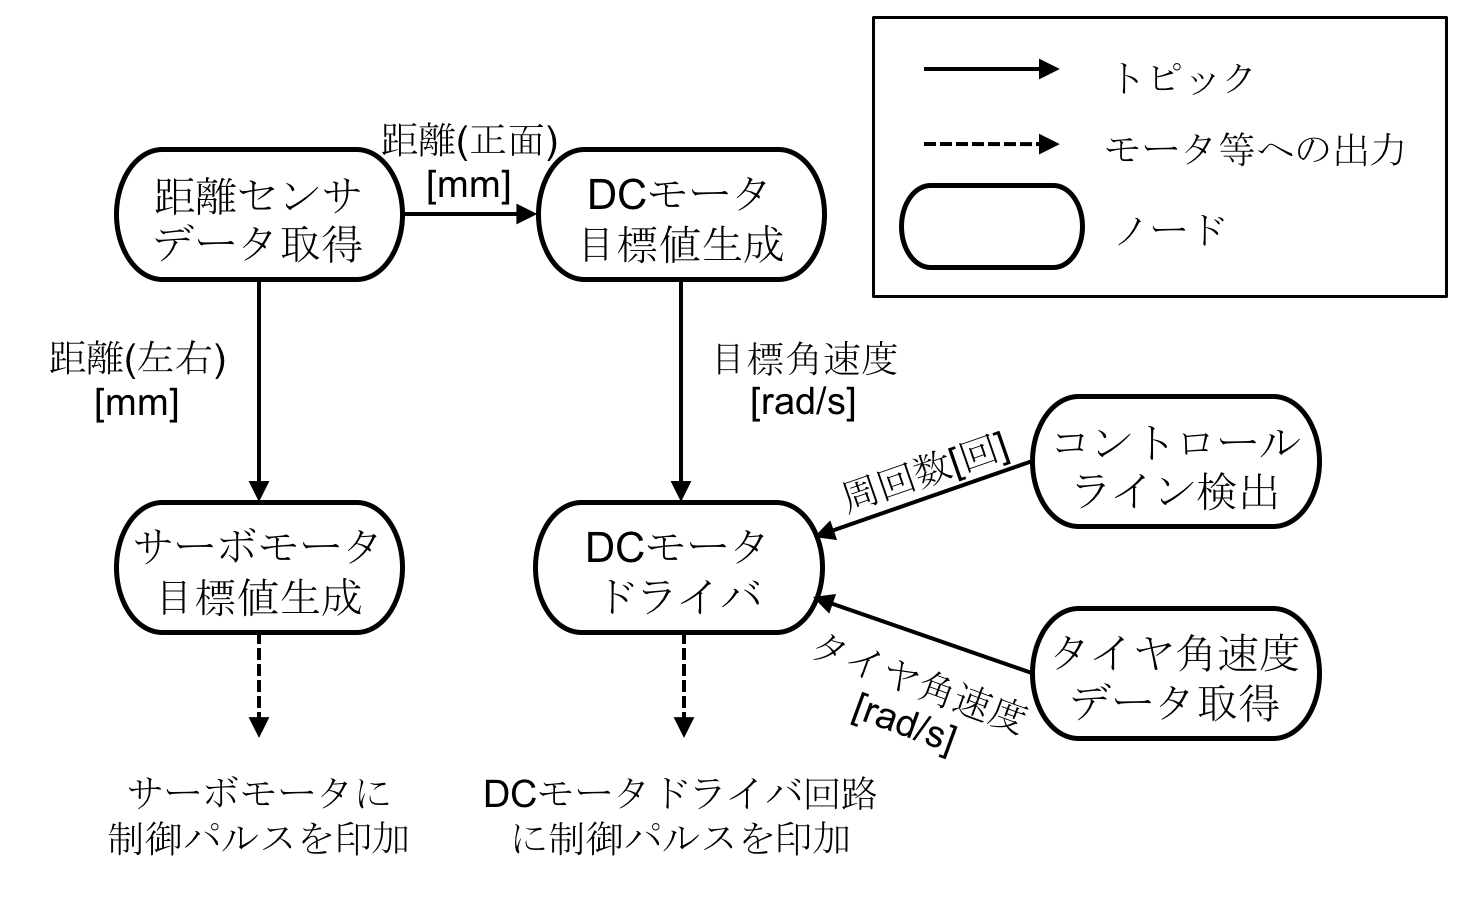
\includegraphics[width=0.8\hsize]{picture/eps/ros_nodes.eps}
    \caption{ROSノードとトピックの構成}
    \label{fig::ros_nodes}
\end{figure}

\newpage
\subsection{ROSノードとトピックの構成}
\refig{ros_nodes}に開発するROSノードとトピックの構成を示す.各ノードの役割は次の通りである.
\begin{description}

    \item[距離センサデータ取得] \mbox{} \\
      ロボカーの前方及び両側面に設置した距離センサからシリアルバス規格の一つである$\mathrm{I^2C}$を介して距離データを$\mathrm{[mm]}$単位で取得し外れ値処理や正規化を施した後にPublishする.
    \item[コントロールライン検出] \mbox{} \\
      ロボカーの後方下部に設置したフォトリフレクタによってコントロールラインを通過した回数をカウントしPublishする.

    \item[タイヤ角速度データ取得] \mbox{} \\
      ロボカーの後方に設置したロータリーエンコーダによって計測したタイヤの回転角を基に,タイヤの回転角速度を算出してPublishする.

    \item[DCモータ目標値生成] \mbox{} \\
      ロボカーの前方方向の距離データをSubscribeし,それをもとにDCモータに与える目標値を生成してPublishする.

    \item[ドライバ] \mbox{} \\
      DCモータに与える目標値,ロボカーの両側面の壁との距離,タイヤの角速度,周回数をSubscribeし,サーボモータの目標値を生成して,サーボモータを駆動させる.また,DCモータを目標値に追従するようなPI制御系によって駆動する.さらに,規定の周回数になるとロボカーを停止させる.


  \end{description}

\newpage
\section{機体}
\refig{first}に配布されたロボカー本体の写真をしめす.\refig{fisrt}より本体の前方には前輪を駆動させ機体を旋回させるためのサーボモータを設置している.そして,本体の後方には後輪を駆動させ機体を動かすためのDCモータを設置し,その上にロータリエンコーダを設置した.

次に,\refig{second}に本体の上に設置するパーツの写真を,\refig{third}にその上に設置するパーツの写真示す.\refig{second}より中央にはDCモータを制御するためのモータドライバ,後方には各部品に電力を供給するためのバッテリ,前方にはRaspberry Pi3 model Bに電力を供給するためのモバイルバッテリを設置した.そして,前方と左右にコースの壁の距離を計測するためのPSDセンサを設置した.\refig{third}より,一番上にはRaspberry Pi3 model BとDC-DCコンバータを含めた電気回路を設置している.

そして,現在,配線が\refig{second},\refig{third}よりロボカー本体に他の部品を設置するためにユニバーサルプレートを採用した.その理由は最初に,加工しやすいからである.ユニバーサルプレートは素材がプラスチックで出来ているので切断しやすいという特徴がある.次に,様々な部品の取り外しや設置がやりやすいからである.ユニバーサルプレートには無数の穴が開いているので簡単にボルトとナットに部品を設置できる.また,プラスチックは電気を通しにくいので電気回路の絶縁にもなるからである.

最後に,\refig{forth}にロボカーの背面の写真を示す.\refig{forth}より,現在はまだ設置してないがロボカーの背面にゴールラインを読み取るためのフォトリフレクタを設置する予定である.

\begin{figure}[htb]
\centering
\includegraphics[width=0.5\hsize]{picture/eps/one.eps}
\caption{ロボカー本体}
\label{fig::first}
\end{figure}

\begin{figure}[htb]
\centering
\includegraphics[width=0.5\hsize]{picture/eps/two.eps}
\caption{ロボカー1段目}
\label{fig::second}
\end{figure}

\begin{figure}[htb]
\centering
\includegraphics[width=0.5\hsize]{picture/eps/three.eps}
\caption{ロボカー2段目}
\label{fig::third}
\end{figure}

\begin{figure}[htb]
\centering
\includegraphics[width=0.5\hsize]{picture/eps/four.eps}
\caption{ロボカー背面}
\label{fig::forth}
\end{figure}

\clearpage
\begin{figure}[h]
\centering
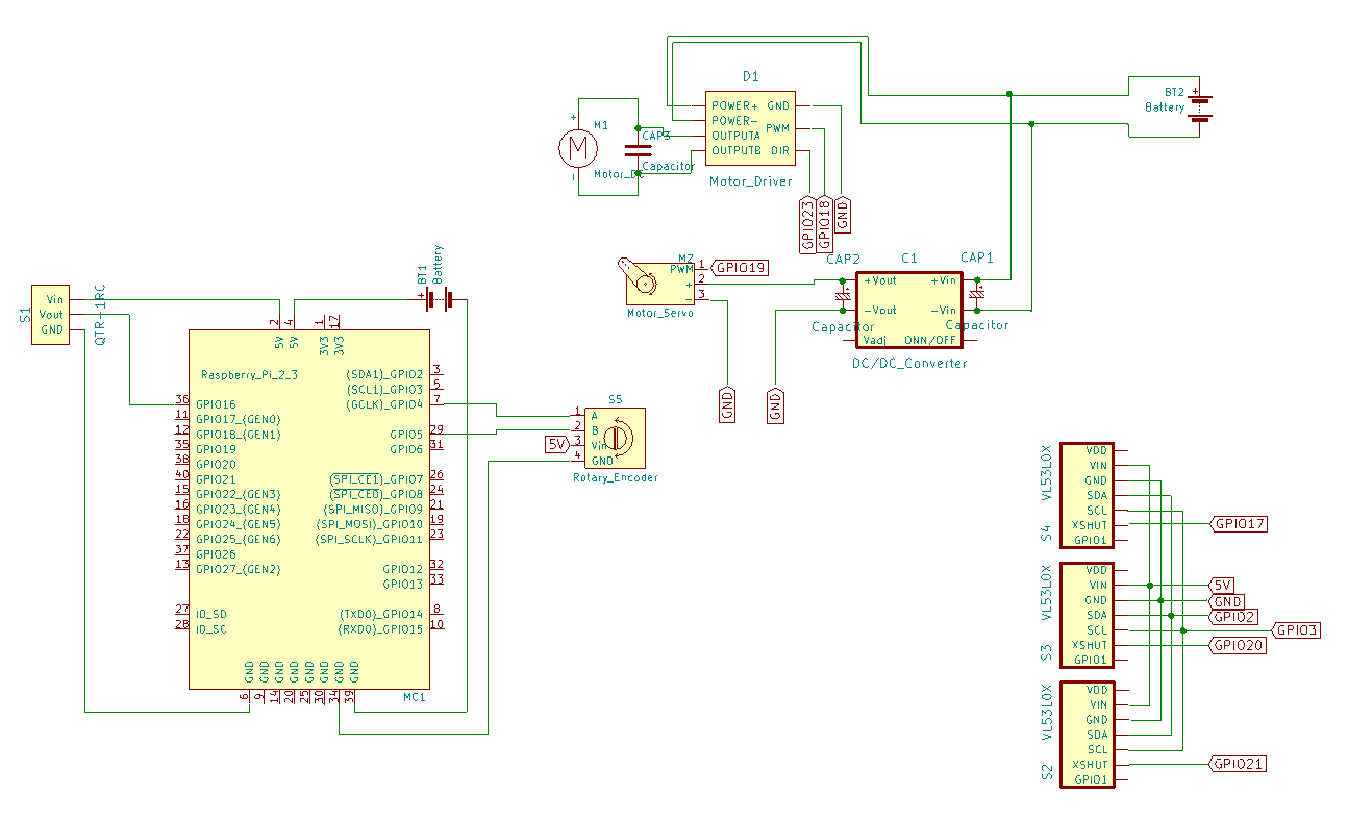
\includegraphics[scale=0.6]{picture/eps/ele_circuit_fig1.eps}
\caption{回路図}
\label{fig::overall_electric_circuit}
\end{figure}
\section{回路設計}
今回設計した回路を\refig{overall_electric_circuit},回路制作に使用した主要な部品の一覧を\reftab{circuit_parts}にそれぞれ示す.さらに各電子部品の仕様や構成について以下に示す.

\subsection{電源回路}
以下に示す仕様のようにRaspberryPi3 Model Bとサーボモータ,DCモータドライバではそれれぞれ定格電圧が異なるため同一の電源を用いることができない.そこで$7.2\unit{V}$バッテリと$5\unit{V}$バッテリの2つを用いている.
$7.2\unit{V}$バッテリはまず分流を行い,一方をDC-DCコンバータを用いて$7.2\unit{V}$から$5\unit{V}$に降圧してサーボモータに供給し,もう片方をDCモータドライバに供給している.$5\unit{V}$バッテリはRaspberryPi3 Model Bに電源を供給している.
\begin{description}
    \item[モータドライバ\textless MD10CR3\textgreater \cite{motordriver}]\mbox{}\\
    \vspace{-5mm}
        \begin{itemize}
            \item モータ電源電圧: DC $5\unit{V}-25\unit{V}$
            \item 最偉大電流  : $13\unit{A}$
            \item ロジック入力電圧: $3.3\unit{V}-5\unit{V}$
        \end{itemize}
    \item[サーボモータ\textless GWS03T/2BBMG\textgreater]\mbox{}\\
    \vspace{-5mm}
         \begin{itemize}
            \item 駆動電圧: DC $4.8\unit{V}-6\unit{V}$
        \end{itemize}
     \item[RaspberryPi3 ModelB\cite{rpi}]\mbox{}\\
     \vspace{-5mm}
         \begin{itemize}
            \item 電源: $5\unit{V}$,$2.5\unit{A}$
        \end{itemize}

\end{description}


\begin{table}
    \caption{電気回路用部品}
    \label{tab::circuit_parts}
    \begin{center}
    \footnotesize
   \begin{tabular}{ | l | l | c || l |}\hline
タイプ               &部品名                                         &数&用途   \\ \hline\hline
マイコン             &Raspberry Pi3 Model B                            &1&制御用           \\ \hline
DCモータ             &RP380-ST                                  &1&後輪モータ駆動用   \\    \hline
モータドライバ          &MD10C R3                                        &1&後輪モータ制御用   \\ \hline
距離センサ            &VL53L0X Time-of-Flight                           &3&距離計測用   \\ \hline
フォトリフレクタ         &QTR-1RC フォトリフレクタ・モジュール              &3&ゴールライン計測用   \\ \hline
DC-DCコンバータ          &BTD05-05S200D                                     &1&降圧用   \\ \hline
コンデンサ                &セラミックコンデンサ$1000\unit{pF}50\unit{V}$ &1&後輪モータのノイズ除去用   \\ \cline{2-4}
                          &OSコンデンサ $10\unit{V}47\unit{\mu F}$                          &2&DC-DCコンバータのノイズ除去用    \\ \hline
ロータリーエンコーダ   &RE30E-500-213-1                                   &1&ロボカーの速度計測用   \\ \hline
バッテリ             &Powers Max 4000 Ni-MH $7.2\unit{V}$                        &1&DCモータ,サーボモータ用の電源\\ \cline{2-4}
                          &$4000\unit{mAh}$ 6CELL ニッケル水素バッテリ                &1&Raspberry Pi3 ModelB用の電源    \\ \hline
サーボモータ           &GWS03T/2BBMG                                &1&ステアリング用   \\    \hline
 
	   \end{tabular} 
	\end{center}
\end{table}


\newpage

\begin{figure}[h!]
\centering
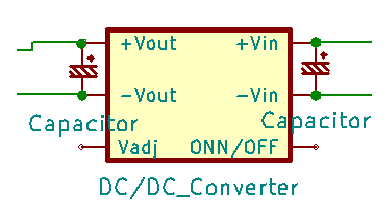
\includegraphics[scale=0.8]{picture/eps/ele_cap.eps}
\caption{DC-DCコンバータの回路図}
\label{fig::ele_cap}
\end{figure}

\subsection{DC-DCコンバータ}
本回路上で降圧を行うためにDC-DCコンバータを用いた.以下にその仕様を示す.DC-DCコンバータは内部でディジタルスイッチングを行っているため,ノイズが多い\cite{dcdc}.本回路ではこのようなノイズ成分を除去するために電解コンデンサ(OSコンデンサ$10\unit{V}47\unit{\mu F}$)を用いた\refig{ele_cap}の回路を作成した\cite{dcdcconverter}.
\begin{description}
    \item[DC-DCコンバータ\textless BTD05-05S200D\textgreater \cite{dcdcconverter}]\mbox{}\\
    \vspace{-5mm}
        \begin{itemize}
            \item 入力電圧: DC $4.5\unit{V}-9\unit{V}$
            \item 出力電圧: $0\unit{mA}-2000\unit{mA}$
            \item 出力電流: $3.3\unit{V}-5\unit{V}$
            \item 効率: 84 \%
        \end{itemize}
\end{description}



\newpage
\section{フォトリフレクタ}
\subsection{使用目的}
フォトリフレクタはロボカーがコースのコントロールラインを読み取るために使用する.本研究室では\refig{photosensor}に示す1RC Reflectance Sensorを用いた.このフォトリフレクタを採用した理由は以下で説明する原理よりAD変換器を使用せずGPIOのディジタル入出力のみで利用可能であるためである.   


\subsection{原理}
このフォトリフレクタの内部の回路図\cite{pololu}を\refig{phses_cir}に示す.はじめにRaspberry Pi mobel BのGPIOピンを出力にした後HIGHを出力し回路内のコンデンサを10マイクロ秒充電する.その後先ほどのGPIOピンを入力に変換する.\\
回路内のLEDが対象物に照射した光の反射光がフォトダイオードに入射することによりフォトダイオードに電流が流れるようになりコンデンサの電圧が減衰する.\\
採用したフォトリフレクタ基板はコンデンサの電圧が一定値より大きければHIGH,小さければLOWという二値出力をするような回路が組み込まれているためパルス幅が長ければコンデンサの電圧減衰時間が長いとみなせる.\\
反射光の反射率が大きければコンデンサの電圧減衰時間が短くなり,反射率が小さければコンデンサの電圧減衰時間が長くなるためパルス波のHIGHの幅の長さにより反射率の大きさを測定することができる.\\
反射率の大きさは色によって異なるのでコンデンサの電圧減衰時間,即ちパルス幅を計測することで対象物の色を判別することができる.

\subsection*{仕様}
\begin{itemize}
\item 作動電圧:5.0[V]
\item 電流電源:17[mA]
\item 最適な検出距離:3.0[mm]
\item 最大検出距離:9.5[mm]
\end{itemize}


\subsection{動作確認実験}
\begin{description}
      \item[色判別] \mbox{} \\
      白色の物体と黒色の物体の表面をフォトレフレクタの3mm上にかざし,物体の色を判別できるか実験した.      
      \item[結果] \mbox{} \\
      色判別の実験において正しく白色の物体と黒色の物体を区別することができた.    
\end{description}

\subsection{今後の実験}
\begin{enumerate}

	\item 実際のコースとコントロールラインの色を判別するために各色のフォトリフレクタが出力するパルス幅について閾値を設定し各色の判定をできるようにする.
	
	\item ロボカーが走行しながらコントロールラインを通過した回数を判定できるようにする.

\end{enumerate}

\begin{figure}[htb]
  \centering
    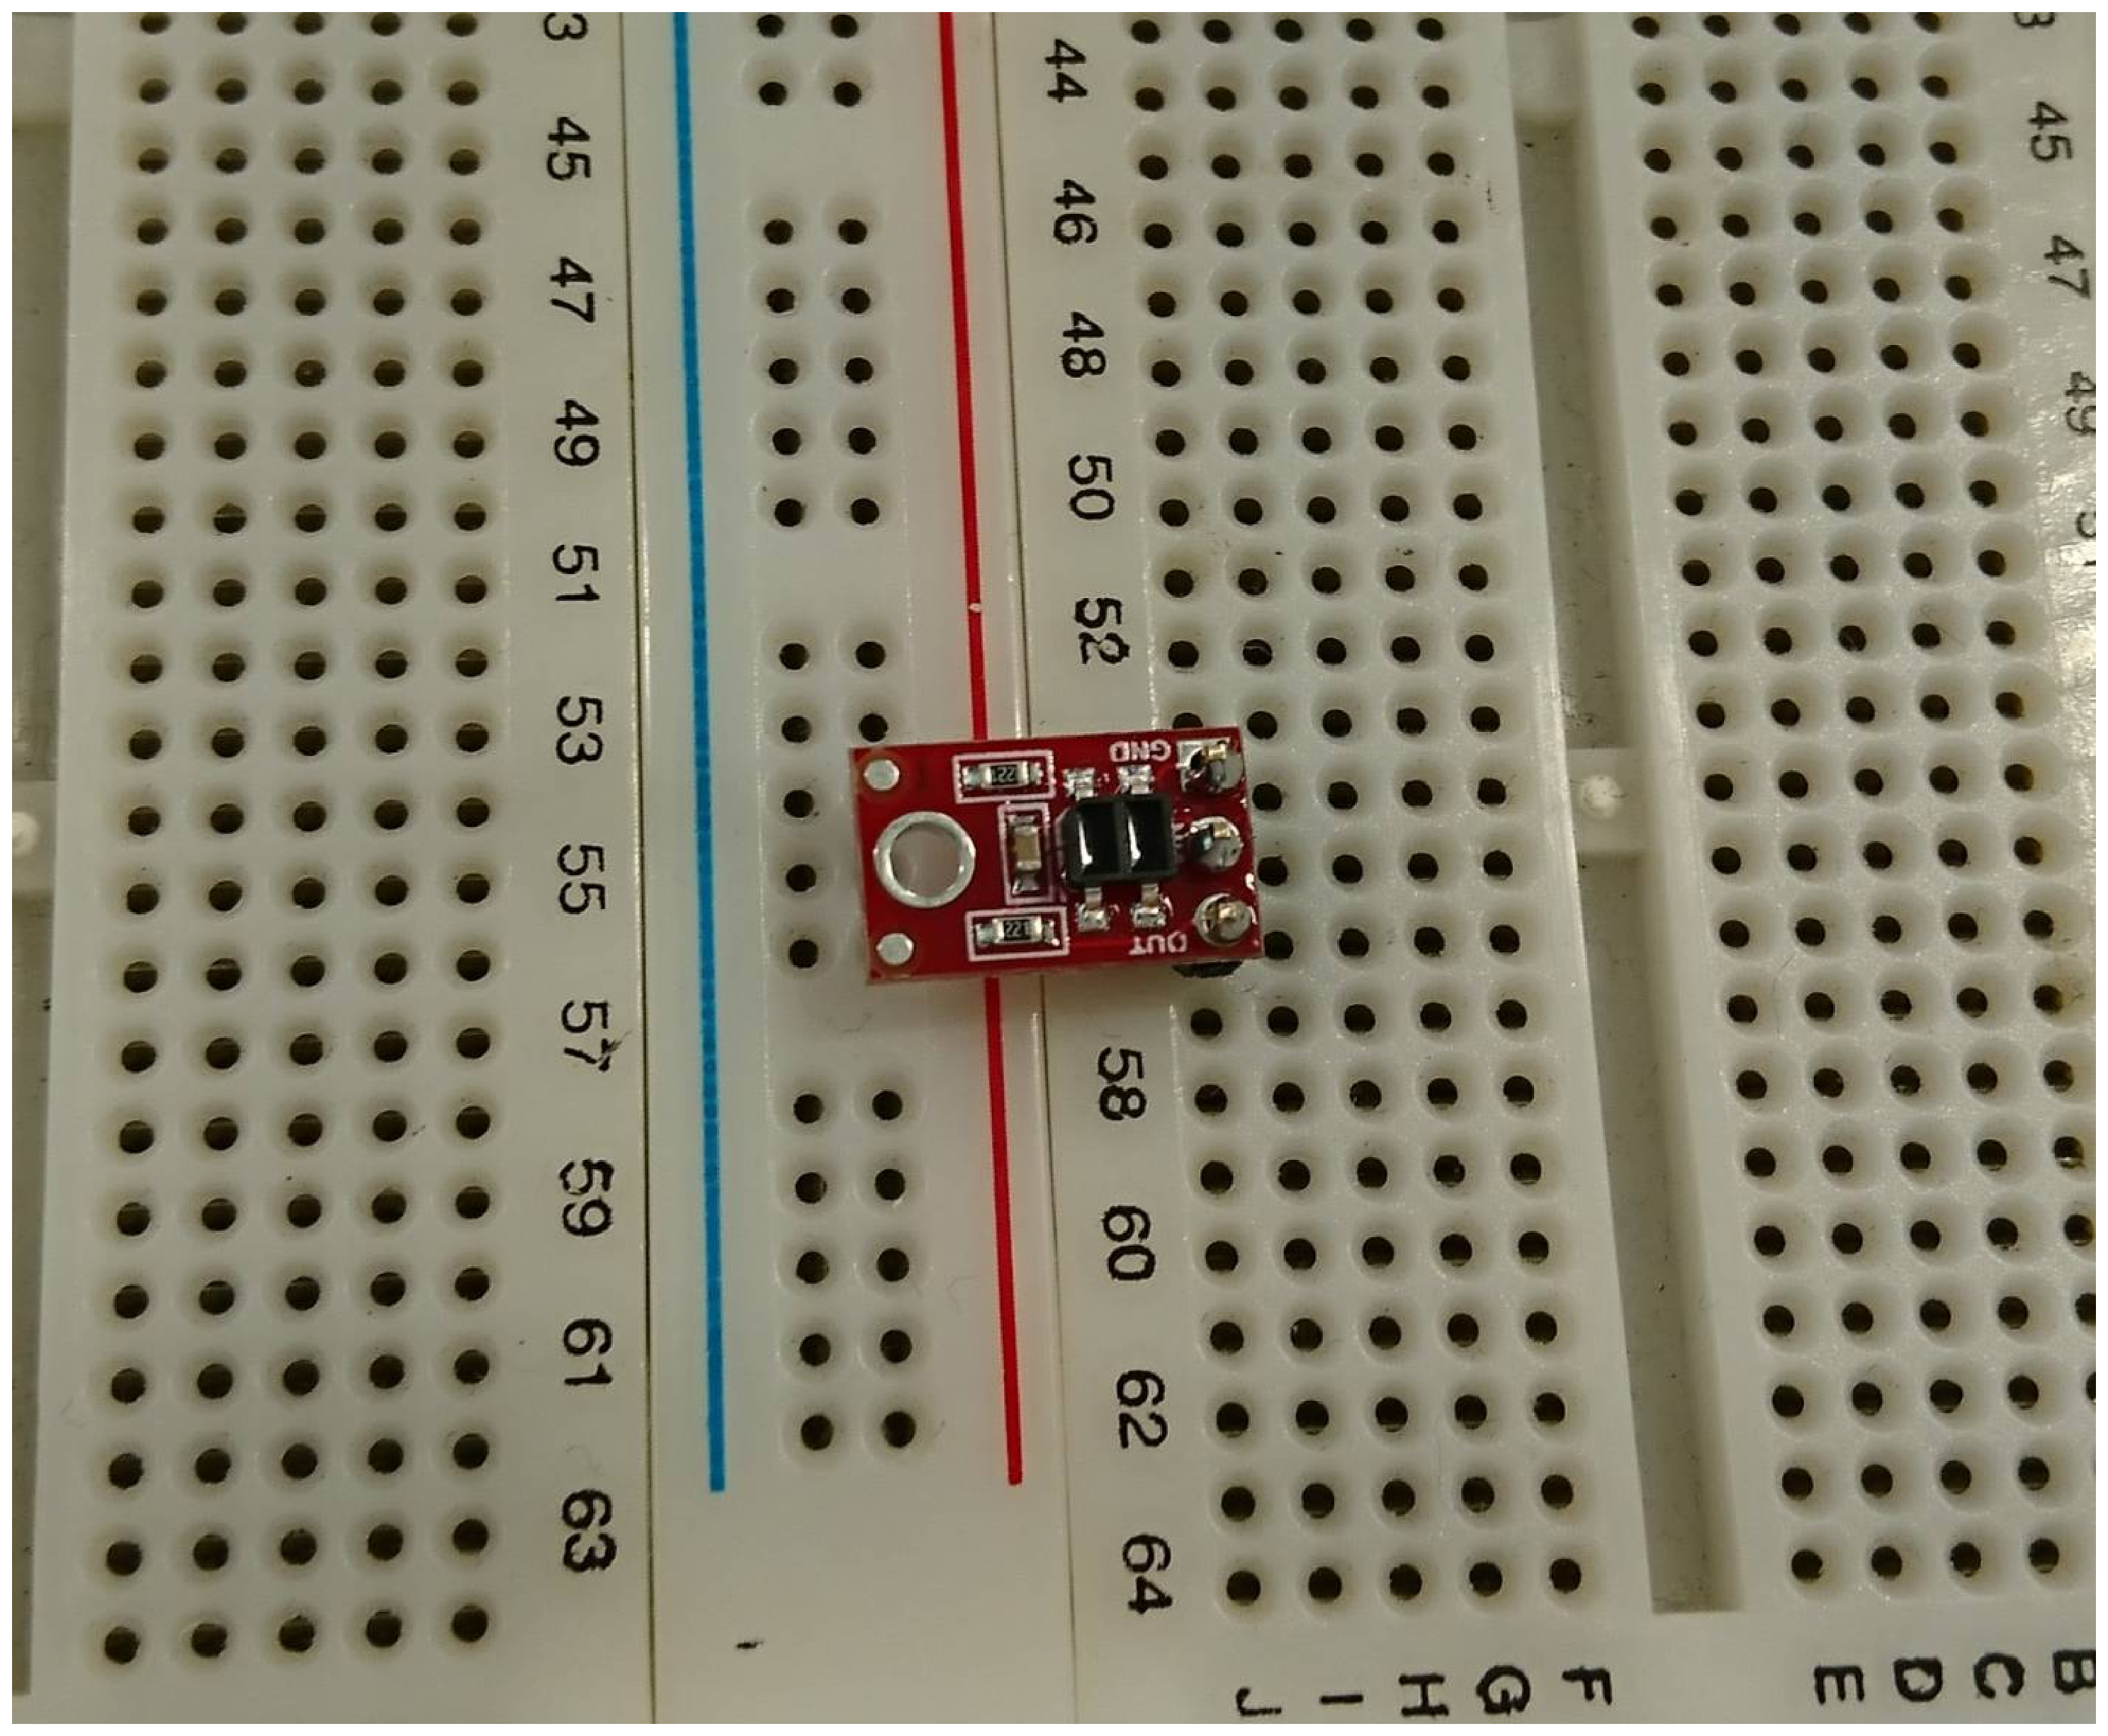
\includegraphics[width=0.5\hsize]{picture/eps/photosensor.eps}
    \caption{フォトリフレクタ}
    \label{fig::photosensor}
\end{figure}

\begin{figure}[htb]
  \centering
    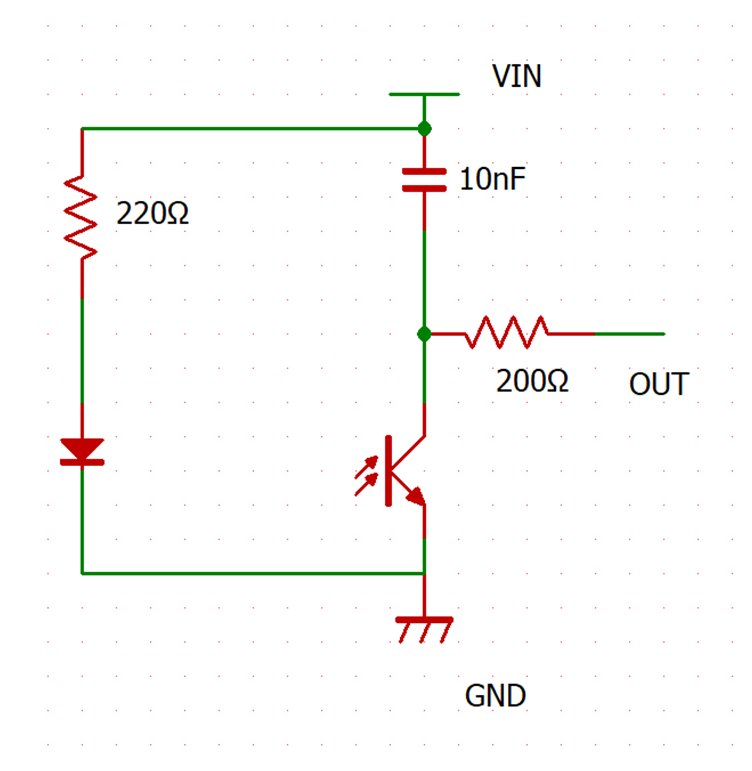
\includegraphics[width=0.5\hsize]{picture/eps/photosensor_circit.eps}
    \caption{フォトリフレクタの内部の回路図}
    \label{fig::phses_cir}
\end{figure}
\newpage
\section{距離センサ}
今回,距離センサとしてPololu VL53L0X Time-of-Flight 距離センサモジュールを採用し,機体の前方に1個,左右に1個ずつの計3個取り付ける.この距離センサモジュールはデジタル$\mathrm{I^{2}C}$インターフェイスを介して距離を測定しており,2.8$\mathrm{[V]}$のリニア・レギュレータと,入力電圧2.6$\mathrm{[V]}$から5.5$\mathrm{[V]}$までに対応する変圧回路を備えている.また,この距離センサモジュールでは赤外線を使用しており,最大2$\mathrm{[m]}$まで計測することができて分解能は1$\mathrm{[mm]}$である.\refig{tof_sensor}にToFセンサの外観を示す.また,以下に仕様を記す\cite{tof_sensor1}.

\begin{itemize}
 \item 動作電圧: 2.6$\mathrm{V}〜5.5\mathrm{V}$
 \item 消費電力: 10$\mathrm{mA}$(通常動作時の平均値)
 \item 検出範囲: 3$\mathrm{cm}〜200\mathrm{cm}$
 \item 重量: 0.5$\mathrm{g}$ (ピンヘッダを除く)
 \item 出力フォーマット$\mathrm{I^{2}C}$: 16ビット読み込み(ミリメートル)
 \item ピンピッチ: 2.54$\mathrm{mm}$ 
\end{itemize}


\subsection{ToF方式}
ToFとはTime-of-Flightの省略形であり,反射光の時間から距離を計算するので,反射光の強度で距離を計測する一般的な測距センサと異なり,測定対象の色や表面状態に依存せずに距離を計測することが可能であり,安定して高フレームレートで測定が可能である\cite{tof_sensor1}.

\begin{figure}[htb]
  \centering
  \includegraphics[width=0.5\hsize]{picture/eps/tof.eps}
  \caption{ToFセンサの外観}
  \label{fig::tof_sensor}
 \end{figure}

\begin{figure}[htb]
  \centering
  \includegraphics[width=0.5\hsize]{picture/eps/tof_experiment_place.eps}
  \caption{ToFセンサの実験装置の外観}
  \label{fig::experiment_place}
\end{figure}

\subsection{$\mathrm{I^{2}C}$}
ここで距離センサモジュールの中で使われている$\mathrm{I^{2}C}$(Inter-Integrated Circuit)について説明する.$\mathrm{I^{2}C}$はフィリップス社で開発されたシリアスバスである.$\mathrm{I^{2}C}$の特徴としては,バス・ラインがシリアル・データ・ライン(SDA)とシリアル・クロック・ライン(SCL)の2本のみという簡単な構造の双方向性バスとなっていること,バスの静電容量が400$\mathrm{pF}$以下であれば,1つのバス上にICをいくつでも接続させることが可能であることなどが挙げられる.また,今回のRCRにおいては$\mathrm{I^{2}C}$インターフェイスを介して値を受け渡すのでA/D変換を行わずに測定した距離の値を受け渡すことができるという利点がある\cite{i2c}.

\subsection{ToFセンサの特性}

\subsubsection{特性実験方法}
ToFセンサの特性実験を行うために,\refig{experiment_place}のような実験装置を準備した.ToFセンサとダンボールの壁が平行になるように曲尺で調整しながら,$\mathrm{5cm}〜\mathrm{70cm}$まで$\mathrm{5cm}$ずつToFセンサで測距を5回ずつ行ってそれらの値をRaspberryPi3 Model Bを通じてモニターに表示し,それらの平均をとった.

\subsubsection{特性実験結果}
横軸に距離の真値,縦軸に距離センサで計測した際に出力された値とし,距離センサの特性を\refig{tof_graph}のグラフに示す.\refig{tof_graph}の値より,この距離センサを最小二乗法により同定した式は次式となる.なお,$x$は実距離$\mathrm{[mm]}$,$y$は出力値$\mathrm{[mm]}$である.
\begin{equation}
  y = 0.96x + 36.9 \label{eq::1pf}
\end{equation}

\refeq{1pf}より,この式の逆関数を取ることによって計測した距離から実際の距離を導出することができる.よって$x$を計測して出力された距離$\mathrm{[mm]}$,$f(x)$を実際の距離$\mathrm{[mm]}$とすると次の式となる.

\begin{equation}
  f(x) = 1.04x - 38.4 \label{eq::2pf}
\end{equation}

よって,実際に距離センサでセンシングする際には,\refeq{2pf}によって計測値を実距離へ変換して用いることになる.

\begin{figure}[htb]
  \centering
  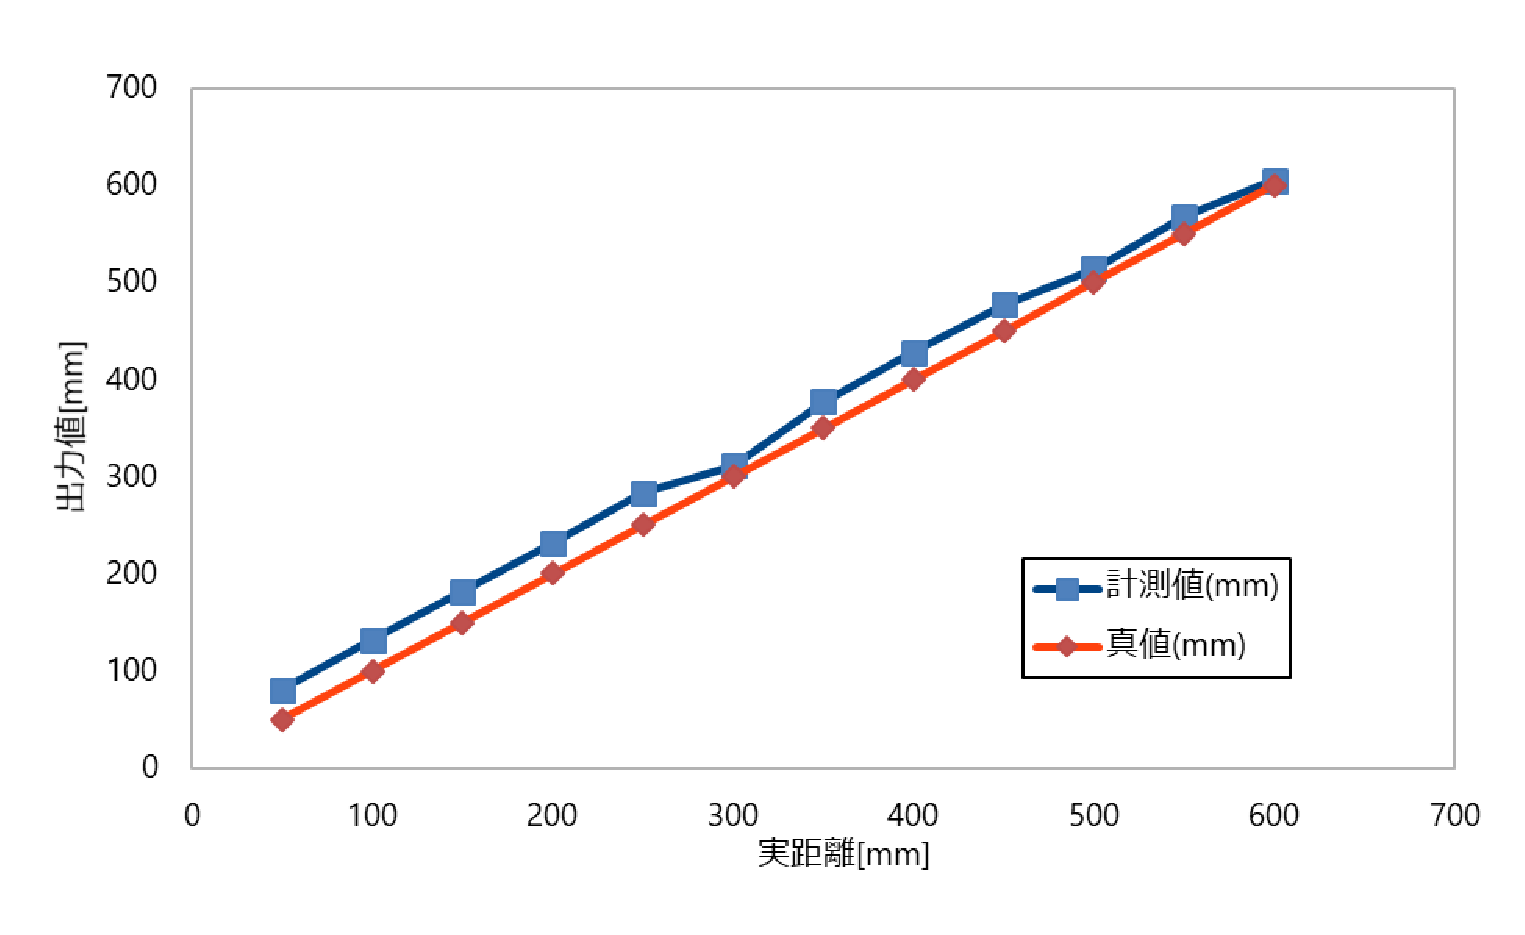
\includegraphics[width=0.5\hsize]{picture/eps/tof_sensor_experiment.eps}
  \caption{ToFセンサの特性}
  \label{fig::tof_graph}
 \end{figure}

\newpage
\section{ステアリング、速度の制御}
  ロボカーがコースを走る際,直進コースでは機体を安定させ可能な限り速く走らせ,カーブに差し掛かったときにはステアリングとステアリングのための減速が必要である.特に,カーブを曲がりきるためにはどれだけのステアリング角と速度にすべきか,またその目標角度に追従させるためにはどのような制御系を構成する必要があるのかを考えなければならない.ここでは,ステアリング角と速度の目標値生成および制御方法について説明する.
 
 
\subsection{RCサーボモータ}
  ロボカーのステアリング角はRCサーボモータの角度により決められる.すなわち,各時点でのRCサーボモータへの目標角度生成と,その目標値に追従させるための制御方法を考える必要がある.

\subsubsection{目標値生成}
  本レースで走行させるロボカーは,機体の左右側面に設置された距離センサにより左右のコースの壁との距離を検出し,その距離の差に応じてステアリング角を変更させる.例えば,右側の壁との距離が左側の壁との距離より大きければステアリング角を時計回り方向に回転させる.ロボカーが直進コースを走行するときに比べ,カーブに差しかかったときとでは\refig{steering_compa}のように左右の壁との距離の差が大きくなる.すなわち,この距離の差が小さいときにはRCサーボモータの角度は小さくなり機体を進行方向に向かせるようにふるまい,大きくなるほど角度を大きくすることでカーブに差しかかった場合に必要なステアリング角を実現することができる.また,機体をコースの中央に位置させるようにステアリングを行わせることができる.
  
  ここで,RCサーボモータはPWM信号に対し\refig{RC_pulse}のような特性をもつ.RCサーボモータでのPWM信号の周期は$16〜23\unit{msec}$であり,その周期中のパルス幅の大きさに比例して角度が決まることがわかる.この特性より,パルス幅$W\unit{msec}$に対して目標角度$\theta_{r}=f(W)\unit{\deg}$とおく.また,左右の壁との距離の差に比例して目標角度を大きくしていくと,距離の差が小さいときに過剰なステアリングを行ってしまうことが考えられる.これが起こると,機体がコースの中央に位置し直進方向を向いているにもかかわらず小さな距離の差に反応してしまい機体の動きを不安定化させてしまう.よって,距離の差の大きさに応じてステアリング角の変化を大きくし,最大角度を超えないようにする必要があるためシグモイド関数$\sigma_{a}(x) $を用いた次式で目標角度$\theta_{r} $を生成することにした.

\begin{equation}  
  \theta = f(W) =f(1.5-2\cdot0.6(\sigma_{a}(x)-0.5)), 
  \sigma_{a}(x)=\frac{1}{1+e^{-ax}}
\end{equation}
ここで,$ a$は定数であり,$ x$は機体の左右のセンサの値の差である.シグモイド関数$\sigma_{a}(x) $は,この式は左右のセンサの値の差によりPWM信号のパルス幅を変えることで目標角度$\theta_{r} $を決定している.\refig{RC_pulse}に示したように,左右のセンサの値の差がなければ$x=0\unit{\deg}$となりパルス幅は$1.5\unit{msec}$となって目標角度$\theta_{r}$は$0\unit{\deg}$となる.右のセンサの値が左のセンサの値より大きい場合を正とすれば,RCサーボモータの角度は右の壁との距離の方が大きくなると時計回りに大きくなり,左の壁との距離のほうが大きくなると反時計回りに大きくなる.定数$a$はシグモイド関数の変化の速さにかかわり,試走実験を通して適切な値とする必要がある.

\subsubsection{構造}
  RCサーボモータは内部でフィードバック制御が行われている.その構造は\refig{RC_construction}に示すとおりである.目標角度に対応するPWM信号を入力すると内部で目標値に追従するように制御が行われる.よって,RCサーボモータの制御については制御系については考えず,目標角度を決めるだけとした.

\begin{figure}[htb]

  \centering
    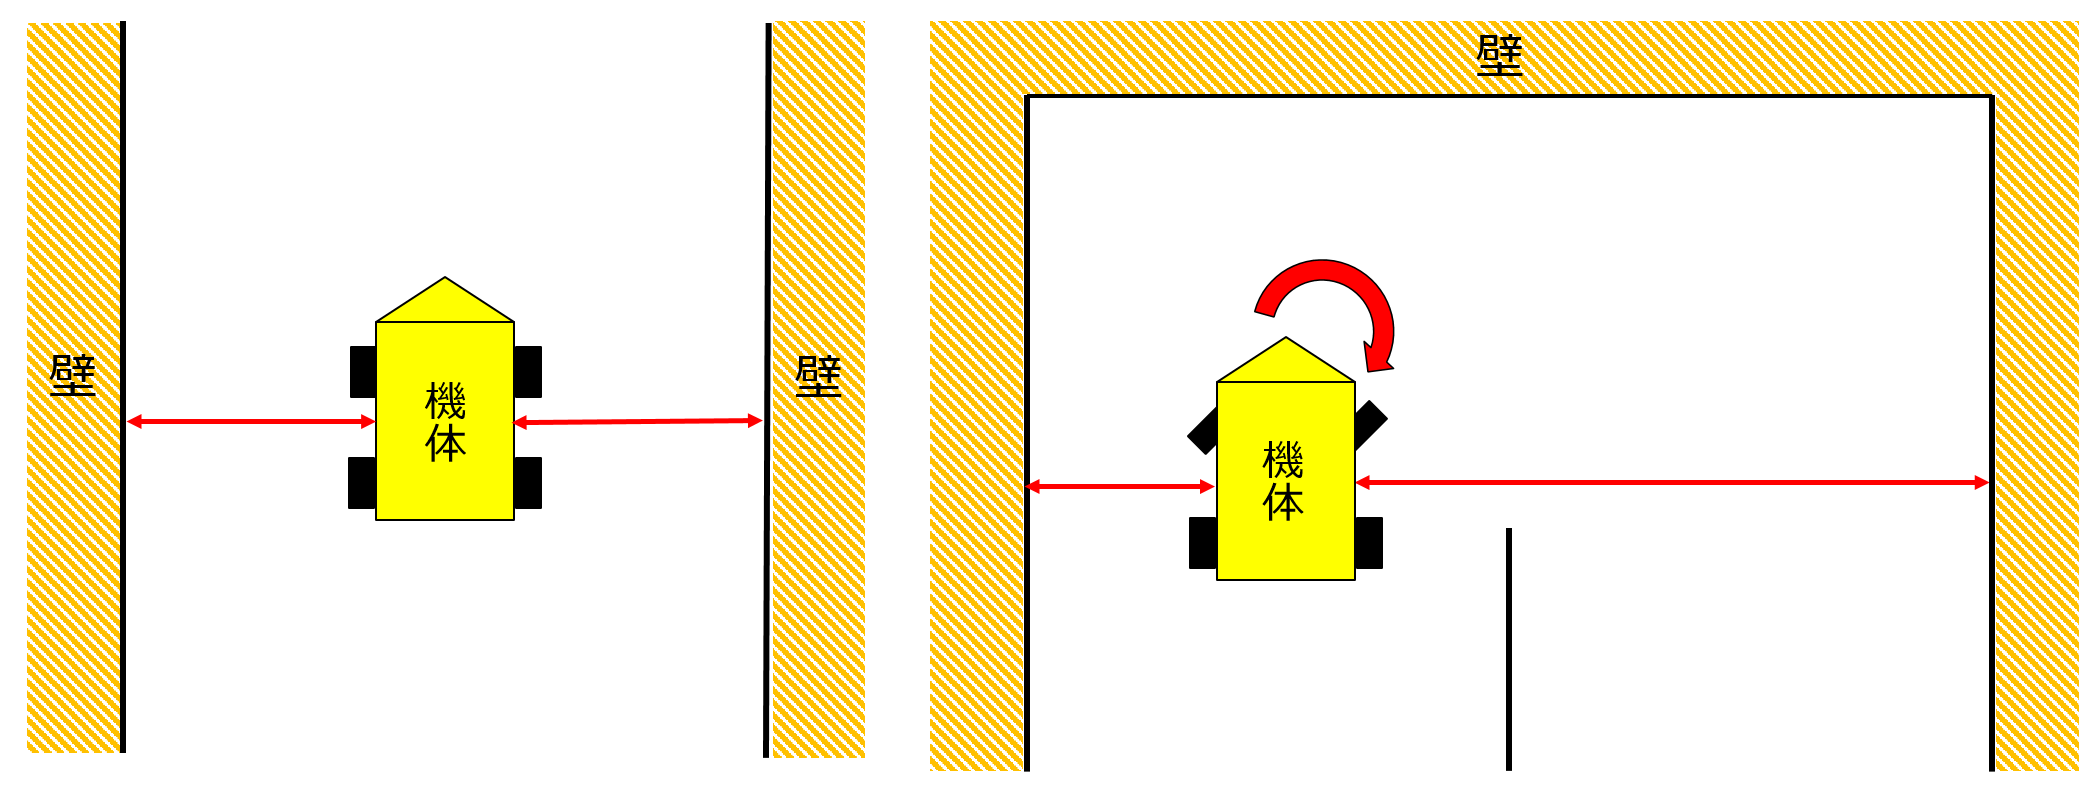
\includegraphics[width=0.7\hsize]{picture/eps/steering_compa.eps}
  \caption{左右の壁との距離の差によるステアリング}
  \label{fig::steering_compa}
\end{figure}  

\begin{figure}[htb]

  \centering
    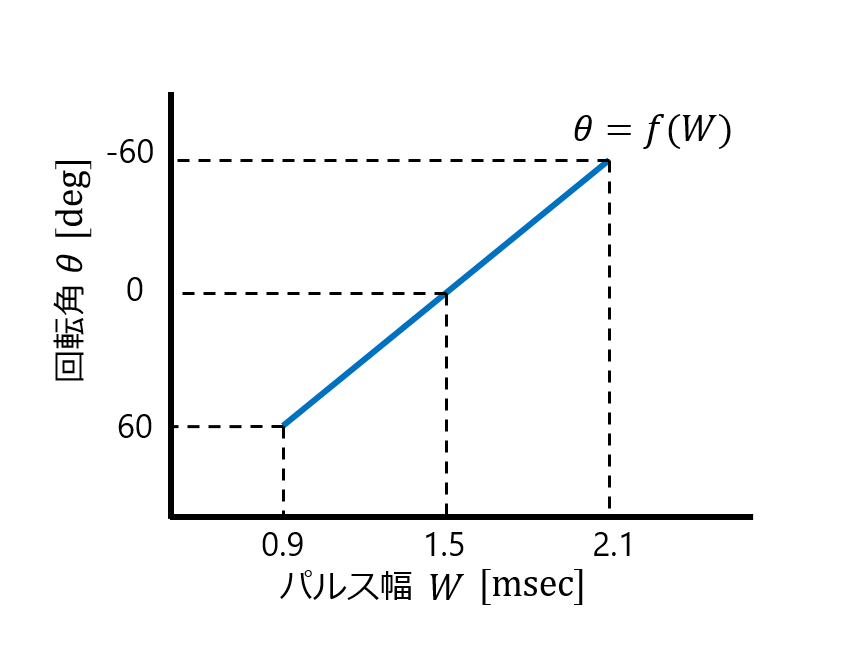
\includegraphics[width=0.5\hsize]{picture/eps/RC_pulse.eps}
  \caption{PWM信号のパルス幅とRCサーボモータの角度の関係}
  \label{fig::RC_pulse}
\end{figure} 
 
 \begin{figure}[htb]

  \centering
    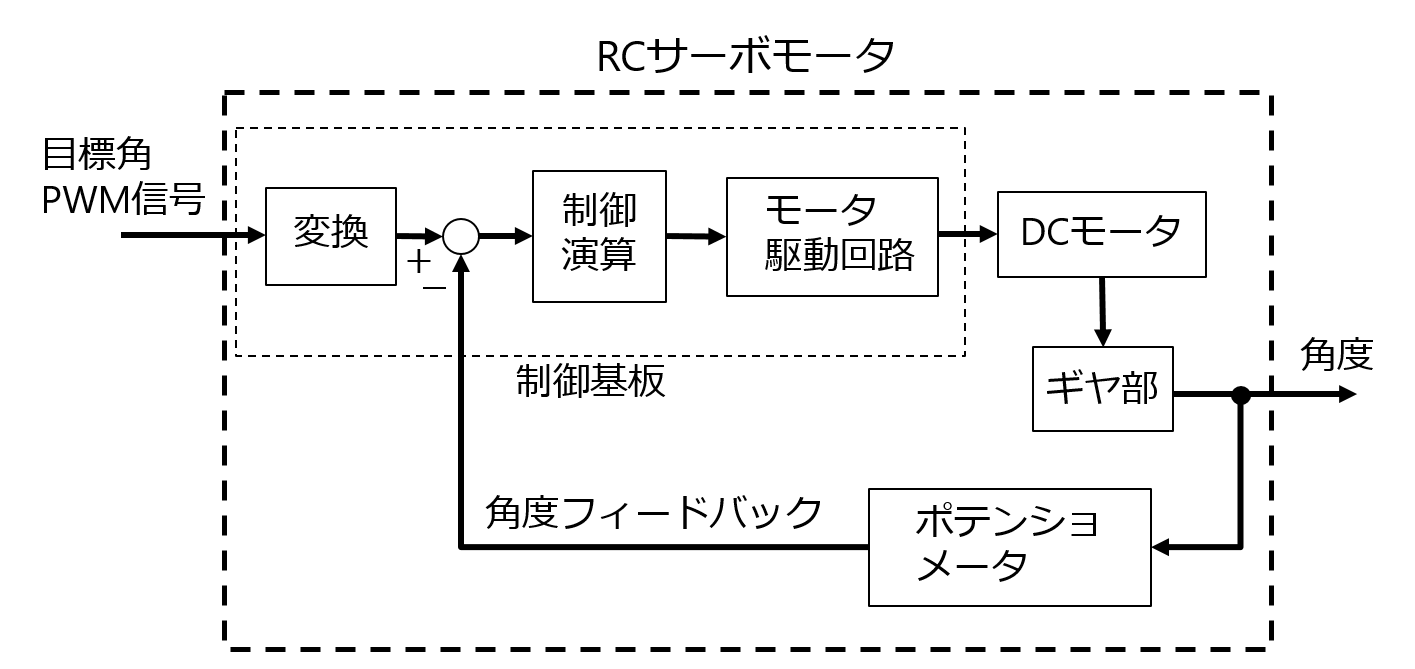
\includegraphics[width=0.6\hsize]{picture/eps/RC_construction.eps}
  \caption{RCサーボモータの制御系}
  \label{fig::RC_construction}
\end{figure} 

 \begin{figure}[htb]

  \centering
    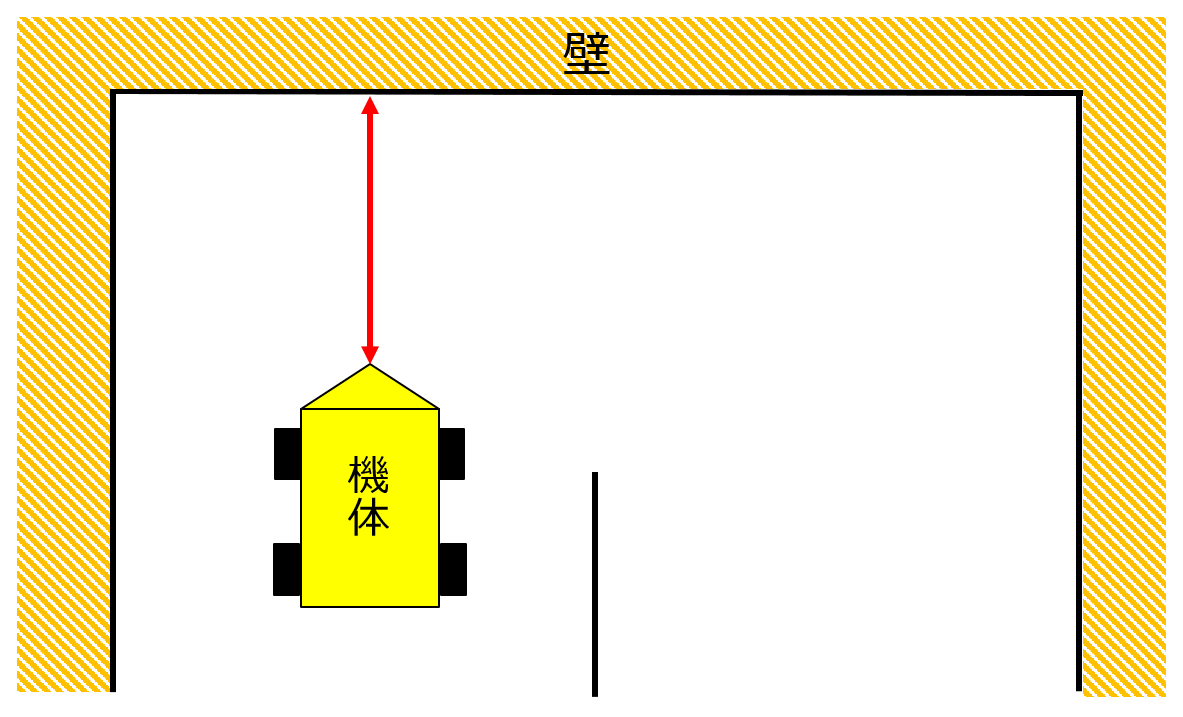
\includegraphics[width=0.4\hsize]{picture/eps/speed_wall.eps}
  \caption{前方の壁との距離に対する速度}
  \label{fig::speed_wall}
\end{figure}

\begin{figure}[htb]
  \centering
    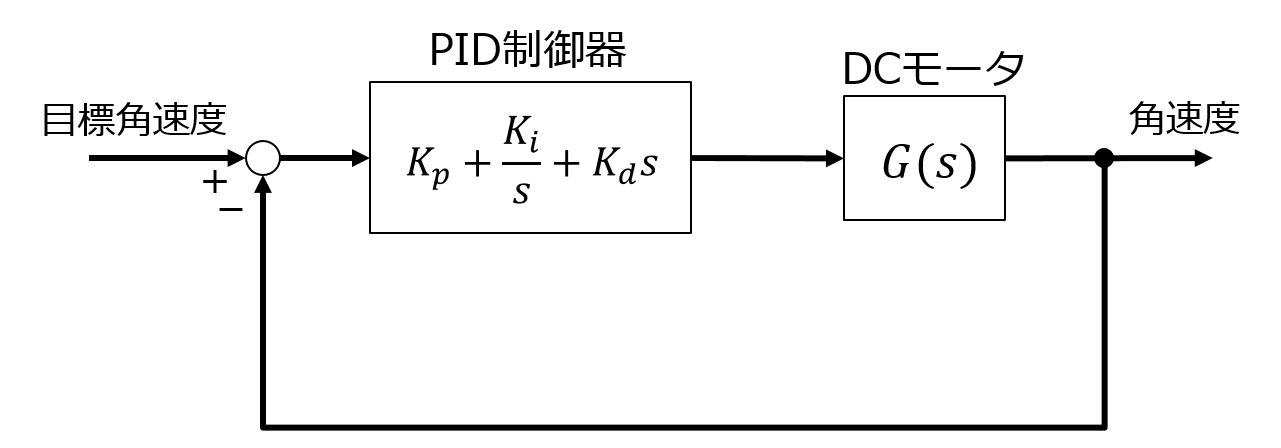
\includegraphics[width=0.5\hsize]{picture/eps/PID_control.eps}
  \caption{DCモータの制御系}
  \label{fig::PID_control}
\end{figure}

\clearpage
\subsection{DCモータ}
 ロボカーの速度はDCモータの回転角速度により決められる.すなわち,各時点でのDCモータへの目標角速度生成と,その目標値に追従させるための制御方法を考える必要がある.


\subsubsection{目標値生成}
 カーブを曲がりきるためには,ステアリングに余裕をもたせる速度が必要である.本レースで走行させるロボカーは,車体の正面に設置されたToFセンサにより前方の壁との距離を検出し,その距離に応じて速度を変化させる.\refig{speed_wall}のようにカーブに差しかかれば正面のコースの壁との距離は小さくなる.すなわち,正面のコースの壁との距離が小さくなるほどDCモータの角速度を小さくすることで,カーブでの減速を実現することができる.壁との距離に比例して目標角速度を生成すると,壁との距離が大きくなるほどDCモータの角速度が大きくなりモータの最大角速度まで大きくなってしまう.DCモータの角速度が最大の状態でロボカーを走らせると,消費電力が大きくなり電源の消耗が速くなる,機体がモータの回転に耐えられないなどの問題が生じる.この問題を解消するためには最大角速度をある値までに抑え,前方の壁との距離が一定以上になるとそれ以上角速度が上がらないようにする必要がある.なおかつ,壁との距離が小さくなれば速度を落としたいので,DCモータの角速度の目標値生成には,RCサーボモータと同様にシグモイド関数$\sigma_{a}(x)$を用いることにした.指定する最大角速度を$\omega_{max}\unit{rad/s} $とすれば,DCモータへの目標角速度$\omega_{r}\unit{rad/s}$は次式で生成される.

\begin{equation}
 \omega_{r}=2\omega_{max}(\sigma_{a}(x)-0.5), 
 \sigma_{a}(x)=\frac{1}{1+e^{-ax}}
\end{equation}

ここで,$a$は定数であり,$x$は前方のセンサの値である.シグモイド関数$\sigma_{a}(x)$は前方の壁との距離に対し増減する.この式を与えれば,壁との距離がどれだけ離れても目標角速度$\omega_{r}\unit{rad/s}$は指定最大角速度$\omega_{max}\unit{rad/s}$に抑えられ,電力消費を抑えることができる.定数$a$はシグモイド関数の変化の速さに関わり,試走実験を通して適切な値に決める必要がある.
\subsubsection{制御系}
  DCモータの制御系は,\refig{PID_control}に示すようにPID制御器を用いた閉ループ系で構成する.PID制御器を用いるのは,DCモータの角速度を目標角速度へ速やかに安定して到達させるためである.$G(s)$はDCモータの入力電圧から出力角速度への伝達関数であり,実験により求める必要がある.これはDCモータの入力電圧に対する出力角速度の応答を同定することで求められる.またPID制御器中の$K_{p}$,$K_{i}$,$K_{d}$は順に比例ゲイン,積分ゲイン,微分ゲインである.求めた伝達関数$G(s)$のボード線図から,ゲイン余裕,位相余裕などが適切な値になるように,また機体が想定通りの動きをするようにこれらのゲインを調節し,決定する必要がある.

\newpage
\section{物品一覧} 
今回の配布品,引継ぎ品,新規購入品を以下の表に示す.
\begin{table}[h]
	\centering
	\caption{配布品一覧}
	\includegraphics[clip,scale=0.3]{picture/eps/distribution_part.eps}
    \label{distribution}
\end{table}

\begin{table}[h]
	\centering
	\caption{引継ぎ品一覧}
	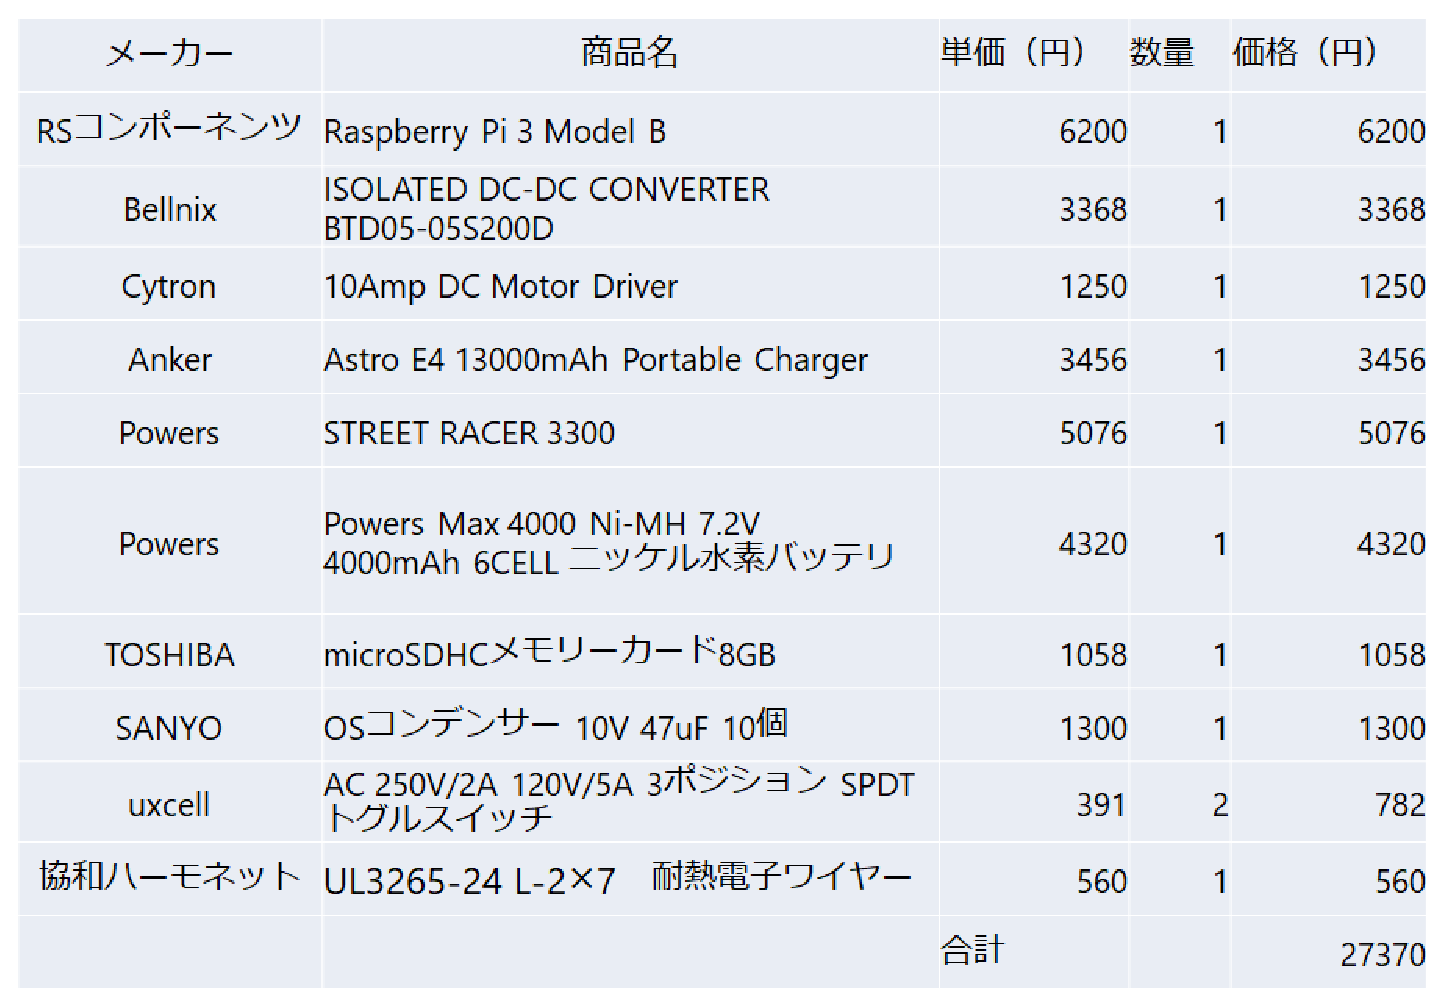
\includegraphics[clip,scale=0.3]{picture/eps/old_part.eps}
 \label{old}
\end{table}

\begin{table}[h]
	\centering
	\caption{購入品一覧}
	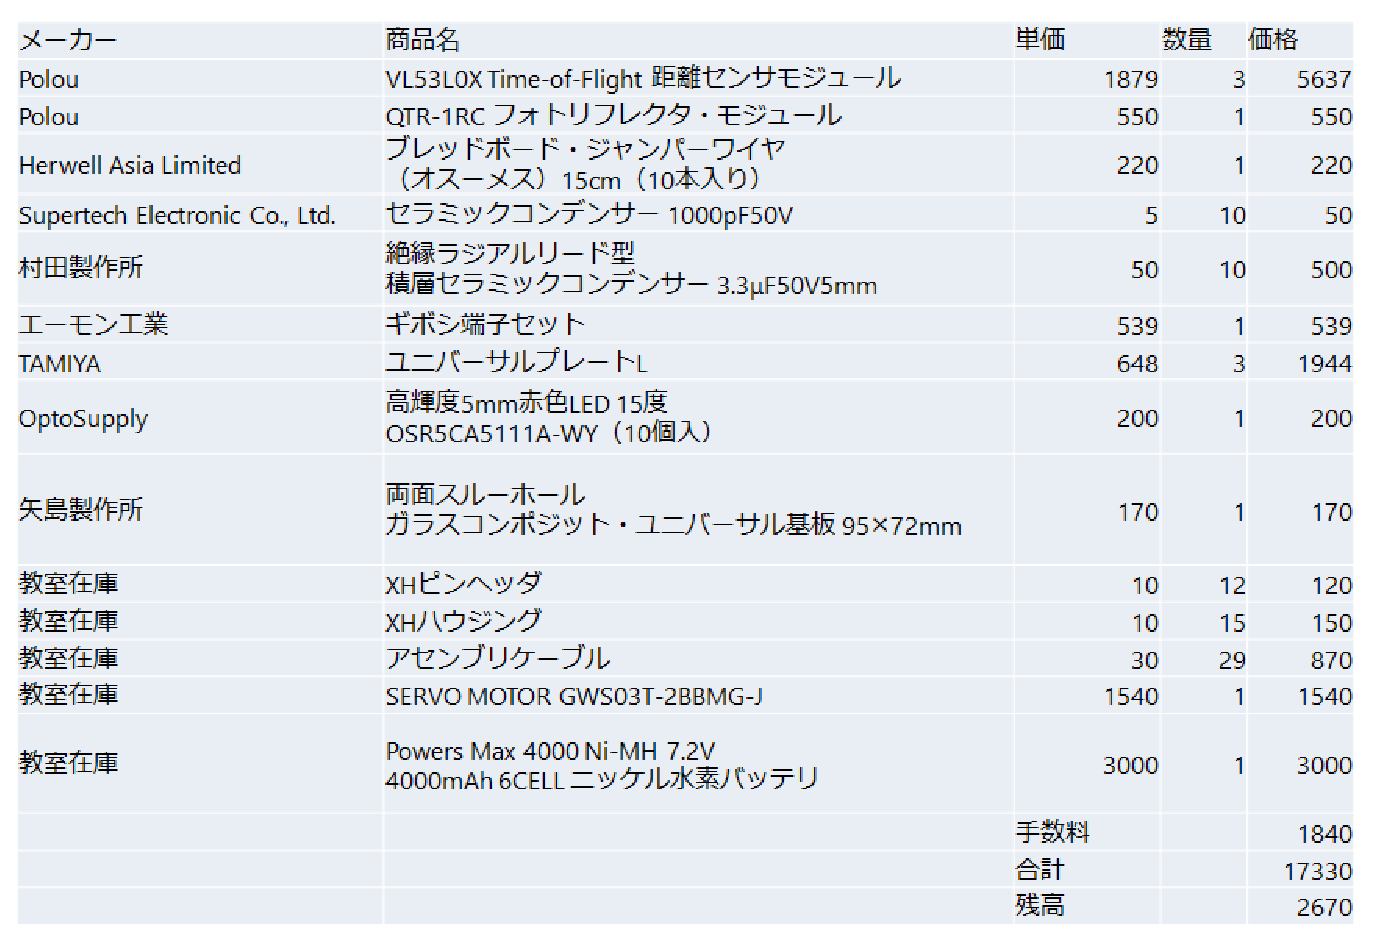
\includegraphics[clip,scale=0.35]{picture/eps/new_part.eps}
    \label{new}
\end{table}



\newpage
\begin{thebibliography}{9}
 \bibitem{kurazume}
    表允晳,倉爪亮,渡邊裕太, "詳説 ROSロボットプログラミング-導入からSLAM・Gazebo・MoveItまで-", 
    Kurazume Laboratory, pp.15-18, (2015).

  \bibitem{ogura}
    小倉崇, "ROSではじめるロボットプログラミング", 工学社, pp.8-10, (2015).
  
  \bibitem{motor} 
  後閑哲也, "作る,できる/基礎入門 電子工作の素", 技術評論社, p181, (2009).
  
  \bibitem{motordriver} 
  Cytron technologies, "MD10C Enhanced 10Amp DC Motor Driver User's Manual Rev2.0 v1.0", 
  \textless https://www.robotshop.com/media/files/PDF/user-manual-md10c-v2.pdf\textgreater , 2018年6月2日アクセス.
  
  \bibitem{R380} 
  MABUCHI MOTOR, "Let's Motorize", 
  \textless https://www.mabuchi-motor.co.jp/motorize/branch/motor/\textgreater , 2018年6月3日アクセス.
  
  \bibitem{dcdcconverter} 
  SWITCH SCIENCE, "10Watt BTD Series", 
  \textless http://www.bellnix.co.jp/pdf/pdf/BTD.pdf\textgreater , 2018年6月2日アクセス.
  
  \bibitem{dcdc} 
  後閑哲也, "作る,できる/基礎入門 電子工作の素", 技術評論社, pp.84-85, p186, (2009).
  
  \bibitem{pololu}
   Pololu\quad Corporation,\quad "QTR-1RC\quad Reflectance\quad Sensor(2-Pack)",
   \textless https://www.pololu.com/product/2459 \textgreater , 2018年6月1日アクセス.
   
  \bibitem{tof_sensor1}
  SWITCH SCIENCE, "Pololu VL53L0X Time-of-Flight 距離センサモジュール"
  \textless https://www.switch-science.com/catalog/2869 \textgreater
  2018年6月1日アクセス.
  
  \bibitem{i2c}
  Philips\quad Semiconductors,\quad "$\mathrm{I^2C}$\hspace{0.5em}バス仕様書バージョン2.1"          
  \textless http://ekousaku.web.fc2.com/doc/I2C.pdf \textgreater
  \quad 2018年6月1日アクセス.
  

\end{thebibliography}

\end{document}
